\documentclass[10pt, compress]{beamer}

\usetheme{m}

\usepackage{booktabs}
\usepackage[scale=2]{ccicons}
\usepackage{minted}

\usemintedstyle{trac}

\title{Introduction to Git}
\subtitle{https://git-scm.com/book/en/v2/}
\date{\today}
\author{Iwan Njoto Sandjaja}
\institute{Petra Christian University}

\begin{document}

\maketitle

\begin{frame}{Version Control - Headache!?}
	
\includegraphics[width=\textwidth*8/10]{images/aspirin}
\end{frame}

\begin{frame}{Version Control - Solution}
	\begin{enumerate}
		\item Local Version Control Systems
		\item Centralized Version Control Systems
		\item Distributed Version Control Systems
	\end{enumerate}
\end{frame}

\begin{frame}{Local Version Control Systems}
	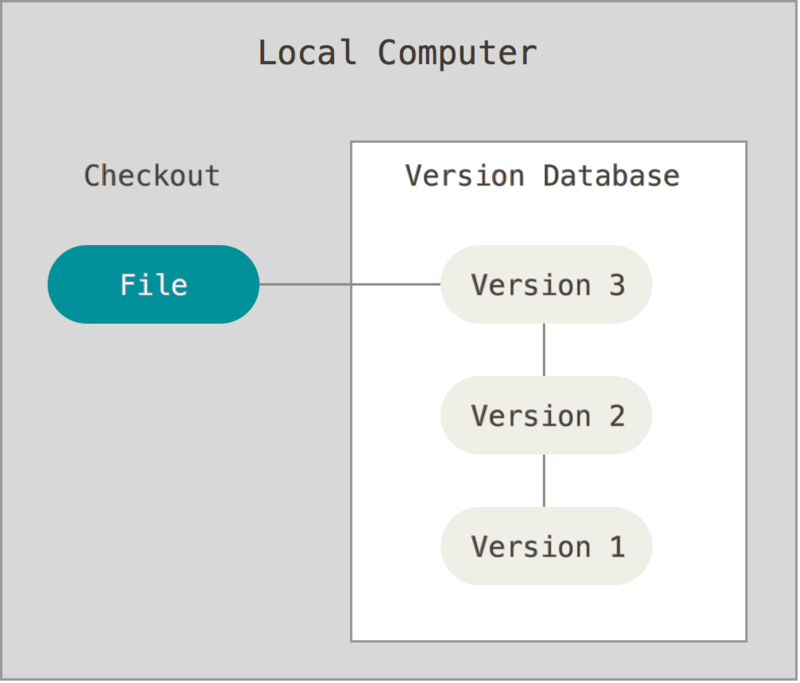
\includegraphics[width=\textwidth*8/10]{images/local}
\end{frame}

\begin{frame}{Centralized Version Control Systems}
	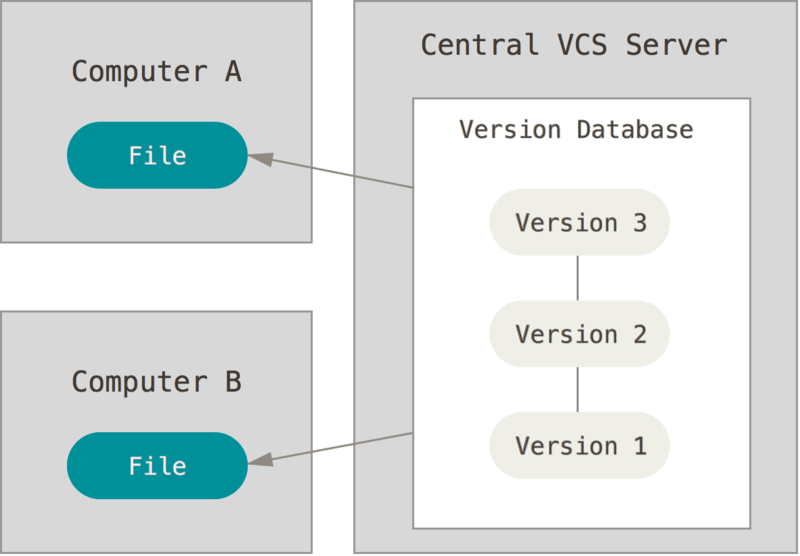
\includegraphics[width=\textwidth*8/10]{images/centralized}
\end{frame}

\begin{frame}{Distributed Version Control Systems}
	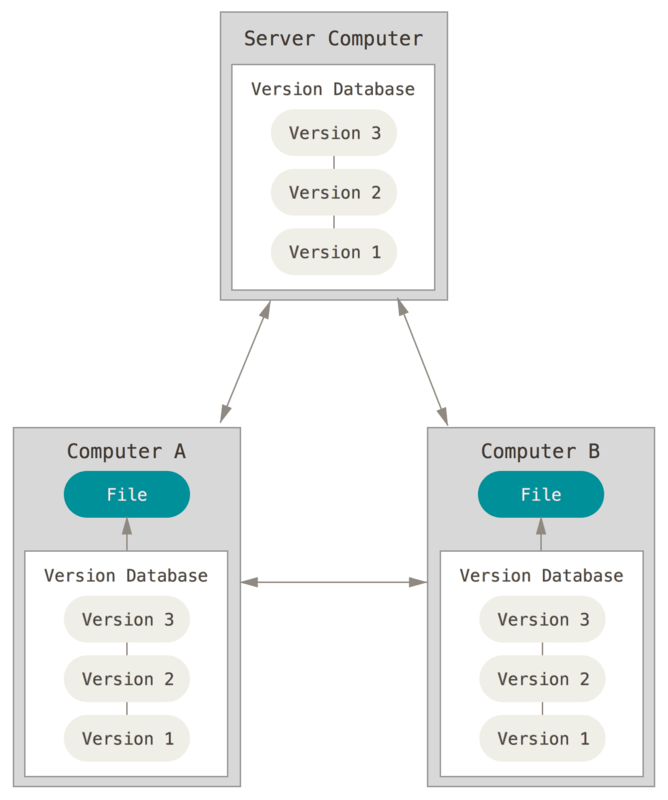
\includegraphics[width=\textwidth*6/10]{images/distributed}
\end{frame}

\begin{frame}{A Short History of Git}
	In 2002, the Linux kernel project began using a proprietary DVCS called BitKeeper.
	
	In 2005, BitKeeper is no longer supporting Linux and Linus Torvalds have to develop a new system with these goals:
	\begin{itemize}
		\item Speed
		\item Simple design
		\item Strong support for non-linear development (thousands of parallel branches)
		\item Fully distributed
		\item Able to handle large projects like the Linux kernel efficiently (speed and data size)
	\end{itemize}		
\end{frame}

\begin{frame}{Git Basics}
	\begin{itemize}
		\item Snapshots, Not Differences
		\item Nearly Every Operation Is Local
		\item Git Has Integrity
		\item Git Generally Only Adds Data
		\item The Three States
	\end{itemize}
\end{frame}

\begin{frame}{Deltas vs. Snapshots}
	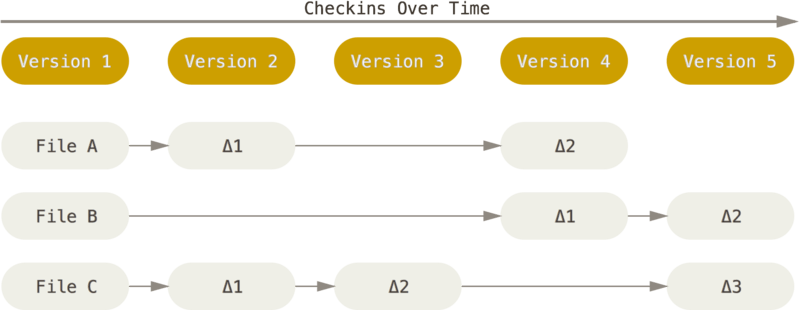
\includegraphics[width=\textwidth*8/10]{images/deltas}
		
	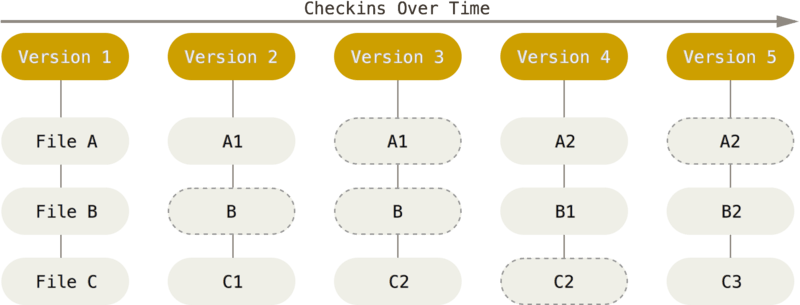
\includegraphics[width=\textwidth*8/10]{images/snapshots}
\end{frame}

\begin{frame}{Modified, Commited, and Staged}
	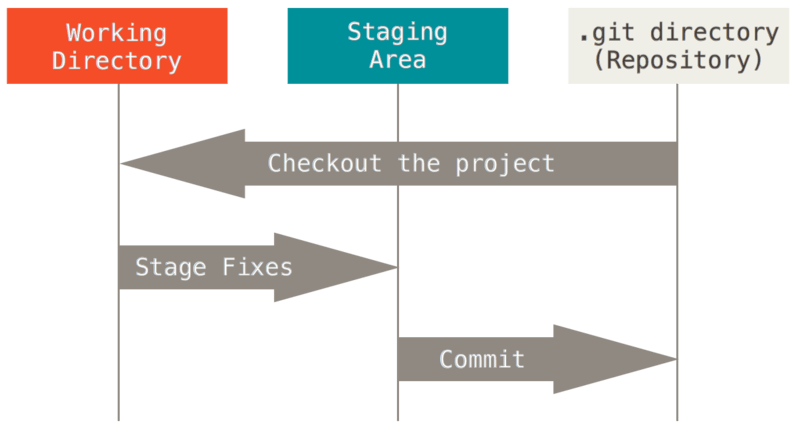
\includegraphics[width=\textwidth]{images/areas}	
\end{frame}


\begin{frame}{Git Workflow}
	\begin{enumerate}
		\item You modify files in your working directory.
		\item You stage the files, adding snapshots of them to your staging area.
		\item You do a commit, which takes the files as they are in the staging area and stores that snapshot permanently to your Git directory.
	\end{enumerate}
\end{frame}

\end{document}
